\documentclass{beamer}

\usepackage{amsmath,amsfonts,amssymb}
\usepackage{graphicx}

\title{Future Visions in Computational Physics}
\subtitle{Towards the Next Paradigm of Scientific Discovery}
\author{Center for Computational Physics, UiO}
\date{AI, Quantum Technology and Neuroscience}

\begin{document}

\frame{\titlepage}

%------------------------------------------------

\begin{frame}{Center for Computational Physics}

As the Center for Computing in Science Education (CCSE) approaches the
conclusion of its mandate in December 2026, we aim to establish a new
center that will carry forward and expand the vision developed within
CCSE. The new center will combine the strong educational foundations
built by CCSE with a renewed emphasis on emerging research directions
in Computational Physics. In particular, it will integrate educational
initiatives with cutting-edge research in artificial intelligence and
machine learning, quantum technologies, and computational
neuroscience. By bringing together these rapidly evolving fields, the
center seeks to prepare students and researchers for the next paradigm
in scientific discovery, where theory, data, and advanced
computational methods are tightly intertwined.

\end{frame}

\begin{frame}{People}
  \begin{itemize}
  \item Gaute Einevoll
  \item Morten Hjorth-Jensen
  \item Anders Malthe-Sørenssen
    \item Many PDs, PhDs and Master of Science students
   \end{itemize}
\end{frame}

\begin{frame}{Motivation}

Computational physics has transformed scientific discovery.

Historically progress relied on

\begin{itemize}
\item improved algorithms
\item increased computational power
\item large-scale simulations
\end{itemize}

Examples include

\begin{itemize}
\item climate modeling
\item lattice quantum field theory
\item materials discovery
\item many-body simulations
\item Neuroscience and many other
\end{itemize}

However, many emerging scientific challenges involve
\textbf{multi-scale and highly complex systems} that
cannot be solved by computational power alone.

\end{frame}


\begin{frame}{Three Pillars of Future Discovery}
\centerline{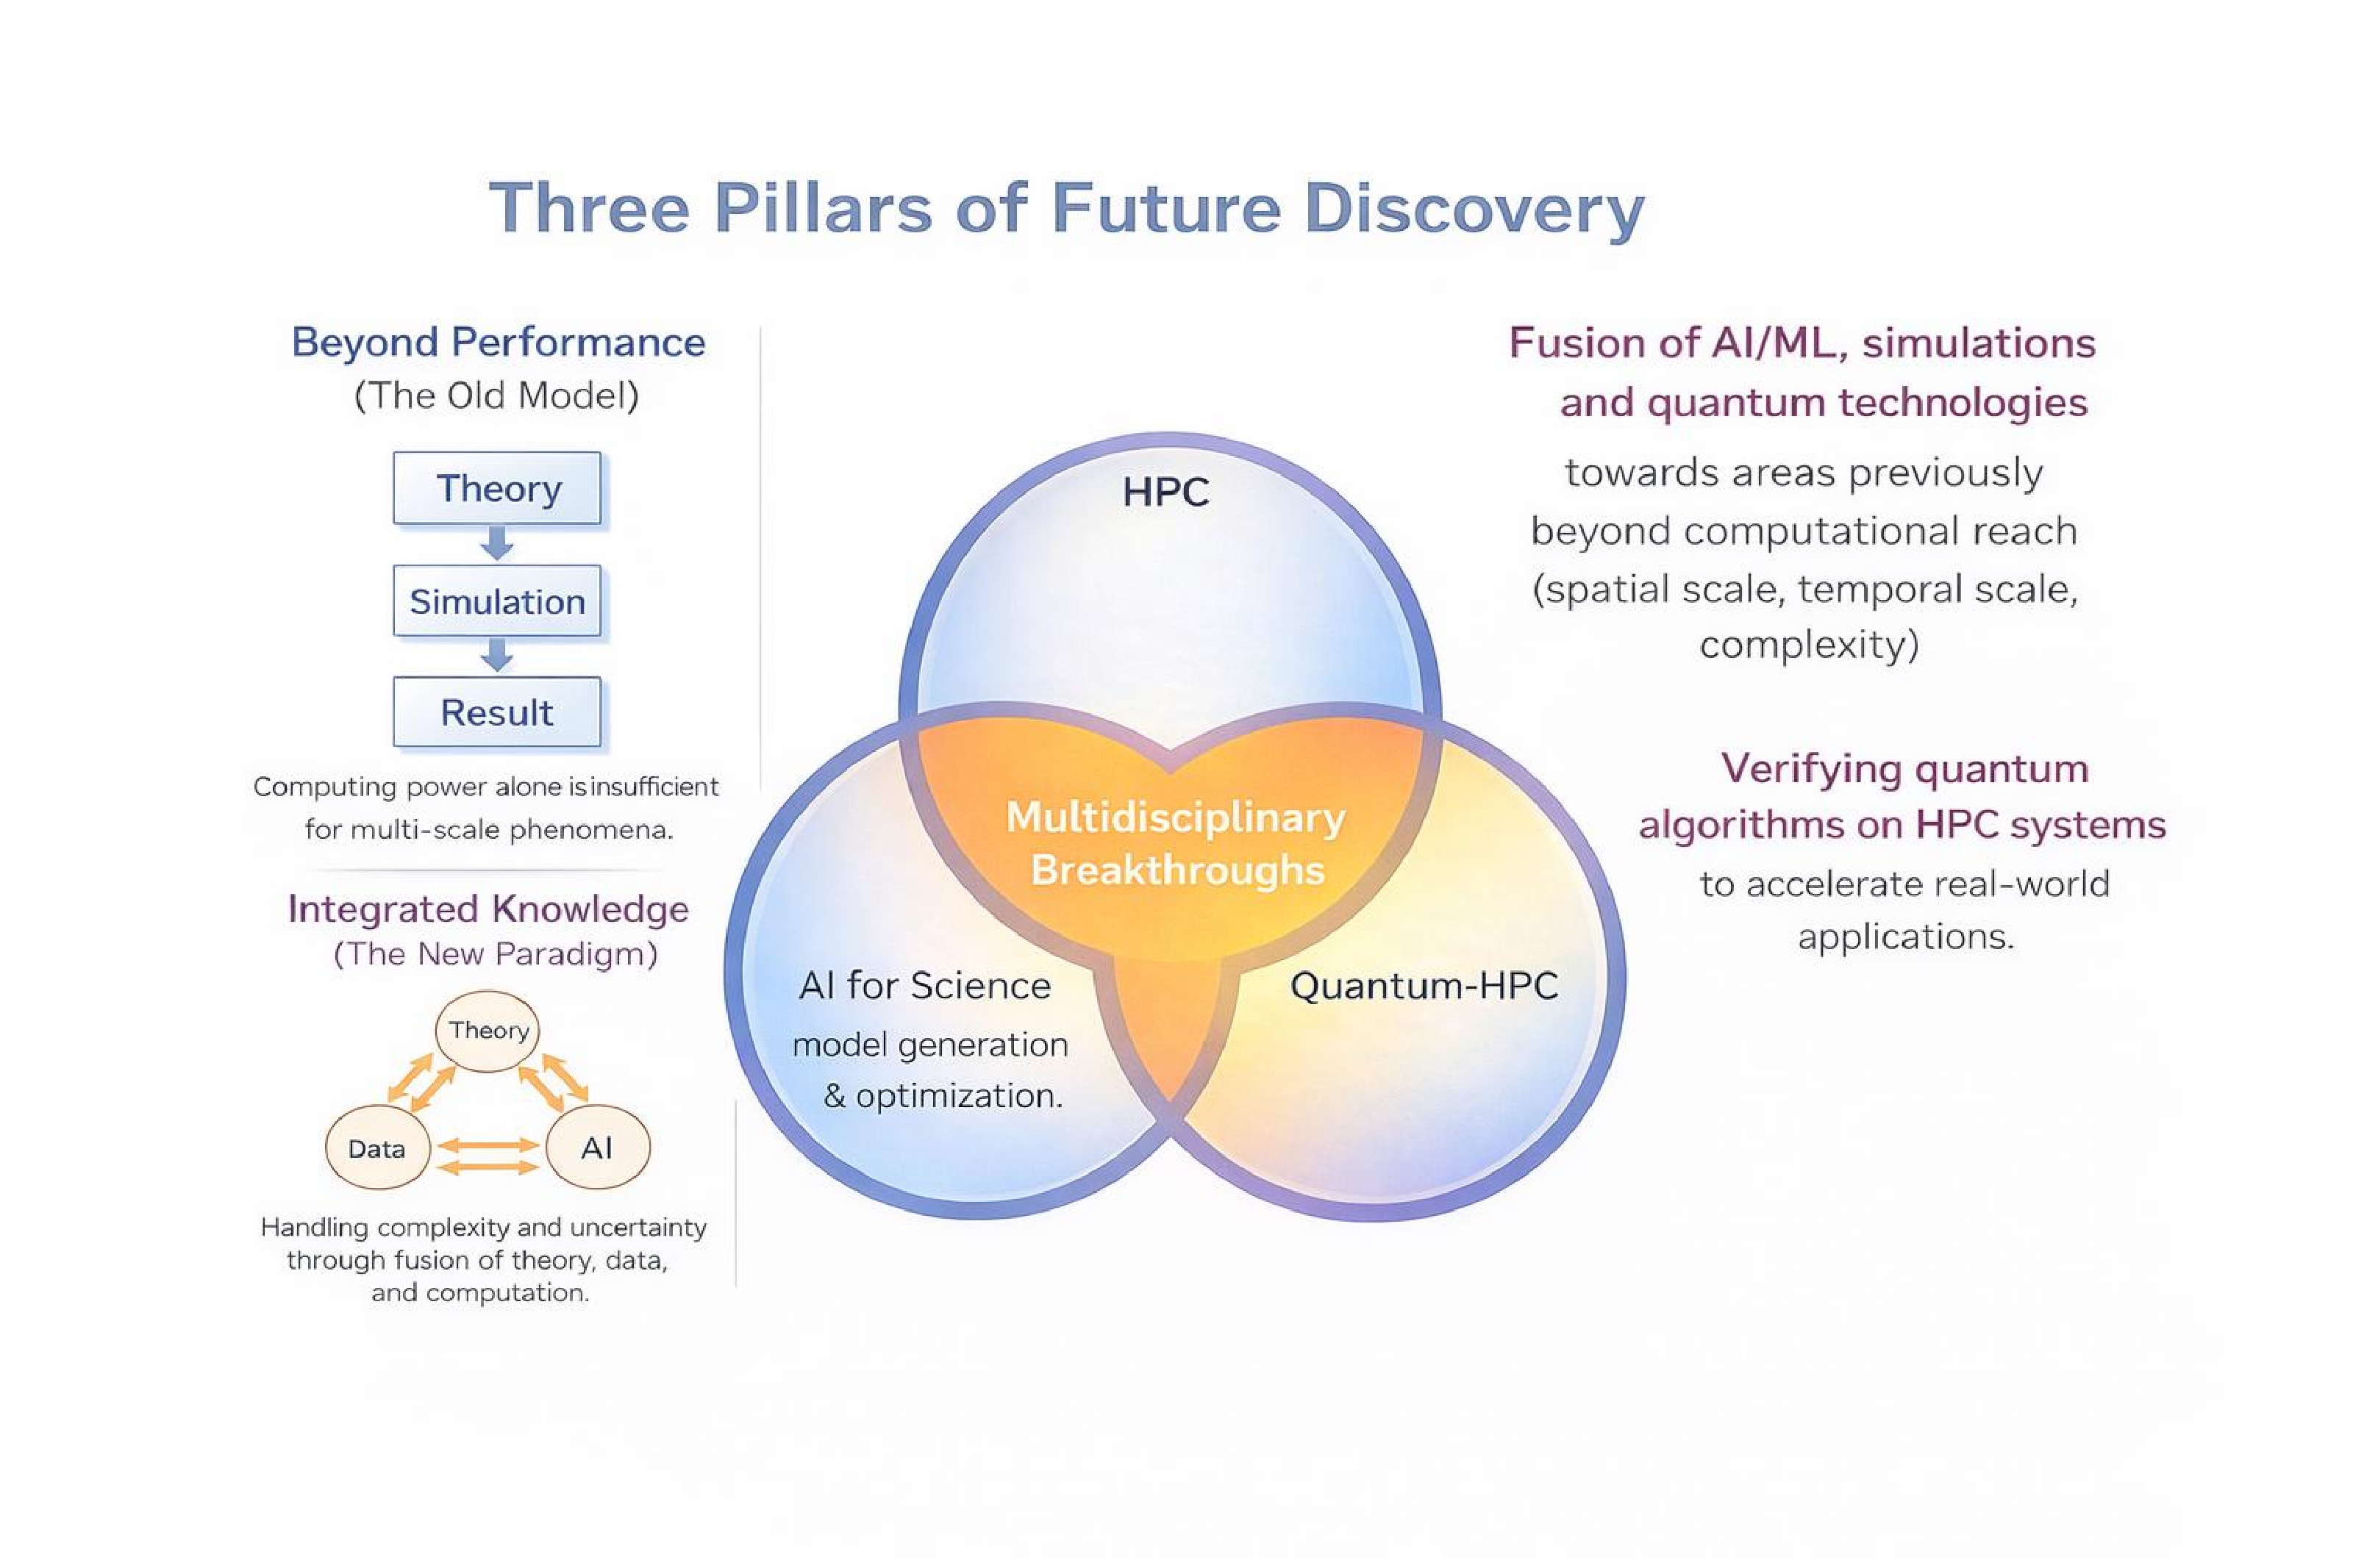
\includegraphics[width=1.0\linewidth]{Futurevision.pdf}}
\end{frame}



\begin{frame}{Three Pillars of Future Discovery}

Future advances in computational physics will rely on
a fusion of three core pillars:

\begin{center}

Theory \\
Simulation / HPC \\
AI/ML and Quantum Technologies

\end{center}

These elements form an integrated ecosystem where

\begin{itemize}
\item theory guides modeling
\item simulations generate data
\item AI extracts patterns
\item quantum technologies extend computational capabilities
\end{itemize}

\end{frame}



%------------------------------------------------

\begin{frame}{The Limits of the Old Paradigm}

Traditional scientific computing relied primarily on

\begin{itemize}
\item numerical algorithms
\item high-performance computing
\end{itemize}

While extremely successful, this approach faces limits:

\begin{itemize}
\item exponential complexity of many-body systems
\item multi-scale physical phenomena
\item large uncertainty in complex models
\item difficulty extracting insight from massive datasets
\end{itemize}

The future requires a new paradigm integrating
\textbf{theory, data, and computation}.

\end{frame}

%------------------------------------------------

\begin{frame}{The New Paradigm}

The emerging paradigm of computational science includes:

\begin{itemize}
\item AI-driven model discovery via LLMs, reinforcement learning, transformers and much more
\item hybrid simulation frameworks
\item quantum computing for specific algorithms, see for example \url{https://arxiv.org/abs/2603.08883}
\item integrated theory–data workflows
\end{itemize}

Key idea:

\begin{center}
\textbf{Fusion of physics-based models and data-driven learning}
\end{center}

This enables exploration of systems that were previously
beyond computational reach.

\end{frame}



%------------------------------------------------

\begin{frame}{Scientific Challenges}

Important challenges in computational physics include

\begin{itemize}
\item strongly correlated quantum systems
\item computational neuroscience
\item climate and Earth system modeling
\item materials for energy technologies
\item complex plasma and astrophysical systems
\end{itemize}

These problems involve

\begin{itemize}
\item many degrees of freedom
\item nonlinear dynamics
\item uncertainty and incomplete data
\end{itemize}

New computational strategies are therefore essential.

\end{frame}

%------------------------------------------------

\begin{frame}{Role of Artificial Intelligence}

Machine learning is becoming a central tool in physics.

Applications include

\begin{itemize}
\item discovery of effective models
\item surrogate models for expensive simulations
\item pattern recognition in experimental data
\item accelerated solution of differential equations
\end{itemize}

Examples:

\begin{itemize}
\item neural-network quantum states
\item physics-informed neural networks
\item machine-learned interatomic potentials
\end{itemize}

AI enables new ways of extracting knowledge from simulations.

\end{frame}

%------------------------------------------------

\begin{frame}{Quantum Computing Opportunities}

Quantum computers may eventually solve problems
that are difficult for classical computers.

Potential applications include

\begin{itemize}
\item quantum chemistry
\item strongly correlated materials
\item optimization problems
\item quantum dynamics simulations
\end{itemize}

Hybrid quantum–classical algorithms such as

\begin{itemize}
\item Variational Quantum Eigensolvers
\item Quantum Approximate Optimization Algorithms
\end{itemize}

are promising early applications.

\end{frame}


%------------------------------------------------

\begin{frame}{Computational Neuroscience and Physics}

Another rapidly growing frontier is computational neuroscience.

The brain can be viewed as a complex physical system consisting of

\begin{itemize}
\item billions of neurons
\item nonlinear dynamical interactions
\item adaptive synaptic couplings
\end{itemize}

Many tools from computational physics are directly applicable:

\begin{itemize}
\item dynamical systems theory
\item statistical mechanics
\item network theory
\item stochastic processes
\end{itemize}

Understanding neural computation therefore represents a natural
extension of computational physics.
\end{frame}

%------------------------------------------------

\begin{frame}{Large-Scale Brain Simulations}

Modern neuroscience increasingly relies on large-scale simulations.

Examples include

\begin{itemize}
\item whole-brain network models
\item cortical microcircuit simulations
\item neural field equations
\item spiking neural networks
\end{itemize}

These simulations require

\begin{itemize}
\item high-performance computing
\item efficient numerical methods
\item large experimental datasets
\end{itemize}

Computational physics methods play a central role in
developing scalable algorithms for these systems.

\end{frame}

%------------------------------------------------

\begin{frame}{Physics-Inspired Models of Neural Systems}

Many neural models are closely related to models in statistical physics.

Examples include

\begin{itemize}
\item Hopfield networks and spin systems
\item Ising models for neural activity
\item mean-field theory of neural populations
\item phase transitions in neural dynamics
\end{itemize}

These approaches allow us to study

\begin{itemize}
\item collective neural dynamics
\item memory formation
\item emergent network behavior
\end{itemize}

from a theoretical physics perspective.

\end{frame}

%------------------------------------------------

\begin{frame}{Machine Learning and Brain-Inspired Computing}

The interaction between neuroscience and machine learning is
a major driver of new computational paradigms.

Research directions include

\begin{itemize}
\item biologically inspired learning algorithms
\item spiking neural networks
\item neuromorphic computing
\item energy-efficient AI hardware
\end{itemize}

Understanding biological neural computation may lead to
new architectures for artificial intelligence.

\end{frame}

%------------------------------------------------

\begin{frame}{Future Research Directions}

Possible interdisciplinary research projects include

\begin{itemize}
\item statistical physics of neural network dynamics
\item AI-assisted analysis of neural recordings
\item multi-scale models of brain activity
\item quantum-inspired algorithms for neural computation
\item hybrid neuromorphic–HPC architectures
\end{itemize}

These directions illustrate how computational physics,
AI, and neuroscience are becoming increasingly connected.

\end{frame}

%------------------------------------------------

\begin{frame}{Vision: Physics of Intelligence}

A long-term scientific goal is the development of a
\textbf{physics of intelligence}.

This program aims to understand

\begin{itemize}
\item how information is represented in neural systems
\item how learning emerges from physical dynamics
\item how complex cognition arises from simple components
\end{itemize}

Combining physics, AI, and neuroscience may therefore
lead to new principles governing complex adaptive systems.

\end{frame}


%------------------------------------------------

\begin{frame}{Integrated Knowledge Discovery}

Future computational physics will rely on
integrated research pipelines:

\begin{enumerate}
\item theoretical model development
\item large-scale numerical simulations
\item machine learning analysis
\item experimental validation
\end{enumerate}

Such workflows allow

\begin{itemize}
\item uncertainty quantification
\item model optimization
\item accelerated scientific discovery
\end{itemize}

This integration represents a major shift in
how computational science is performed.

\end{frame}

%------------------------------------------------

\begin{frame}{Future Research Projects}

Possible research directions include

\begin{itemize}
\item AI-assisted discovery of effective many-body models
\item hybrid quantum-classical algorithms for materials science
\item multi-scale simulations combining atomistic and continuum models
\item physics-informed neural networks for dynamical systems
\item machine-learning accelerated Monte Carlo methods
\end{itemize}

These projects aim to bridge

\begin{itemize}
\item theory
\item simulation
\item data
\end{itemize}

into a unified research framework.

\end{frame}

%------------------------------------------------

\begin{frame}{Conclusion}

Computational physics is entering a new era.

Key trends include

\begin{itemize}
\item integration of theory, data, and computation
\item AI-driven scientific discovery
\item hybrid classical–quantum algorithms
\item large-scale interdisciplinary collaborations
\end{itemize}

The future of computational physics will be defined
not only by faster computers but by

\begin{center}
\textbf{new ways of combining knowledge, data, and algorithms.}
\end{center}

\end{frame}

\end{document}






